%%%%%%%%%%%%%%%%%%%%%%%%%%%%%%%%%%%%%%%%%%%%%%%%%%%%%%%%%%%%%%%%%%%%%
% LaTeX Template: Project Titlepage Modified (v 0.1) by rcx
%
% Original Source: http://www.howtotex.com
% Date: February 2014
% 
% This is a title page template which be used for articles & reports.
% 
% This is the modified version of the original Latex template from
% aforementioned website.
% 
%%%%%%%%%%%%%%%%%%%%%%%%%%%%%%%%%%%%%%%%%%%%%%%%%%%%%%%%%%%%%%%%%%%%%%

\documentclass[12pt]{article}
\usepackage[a4paper]{geometry}
\usepackage[myheadings]{fullpage}
\usepackage{fancyhdr}
\usepackage{lastpage}
\usepackage{graphicx, wrapfig, subcaption, setspace, booktabs}
\usepackage[utf8]{inputenc}
\usepackage[T1]{fontenc}
\usepackage[font=small, labelfont=bf]{caption}
\usepackage{fourier}
\usepackage[protrusion=true, expansion=true]{microtype}
\usepackage[french]{babel}
\usepackage{caption}
\usepackage{sectsty}
\usepackage{url, lipsum}
\usepackage{amsmath}



\usepackage{tikz}
\usepackage[most]{tcolorbox}
\usepackage[pstricks]{bclogo}
\usepackage{pst-blur}




\newcommand{\HRule}[1]{\rule{\linewidth}{#1}}
\onehalfspacing
\setcounter{tocdepth}{5}
\setcounter{secnumdepth}{5}

%-------------------------------------------------------------------------------
% HEADER & FOOTER
%-------------------------------------------------------------------------------
\pagestyle{fancy}
\fancyhf{}
\setlength\headheight{15pt}
\fancyhead[L]{BTS CPRP 1}
\fancyhead[R]{Lycée Le Corbusier}
\fancyfoot[R]{Page \thepage\ sur \pageref{LastPage}}
\fancyfoot[L]{TP - Industrialisation}
%-------------------------------------------------------------------------------
% TITLE PAGE
%-------------------------------------------------------------------------------
 
 

%%%%POUR FAIRE DES EXERCICES INDÉPENDAMMENT DES SECTIONS%%%%
%%%%%%%%%%%%%%%%%%%%%%%%%%%%%%%%%%%%%%%%%%%%%%%%%%%%%%%%%%%%%%%%%%%
\newcounter{exo}
\newenvironment{exo}{\stepcounter{exo}\vspace{0.5cm}{\bfseries Question \theexo\ :}}{\par\vspace{0.5cm}}
%%%%%%%%%%%%%%%%%%%%%%%%%%%%%%%%%%%%%%%%%%%%%%%%%%%%%%%%%%%%%%%%%%%%




\begin{document}
 
\title{ 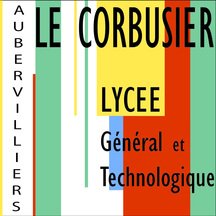
\includegraphics[width=0.18\linewidth]{corbu.jpg} \hspace{2cm} \normalsize \textsc{TP Industrialisation noté \hspace{2cm} 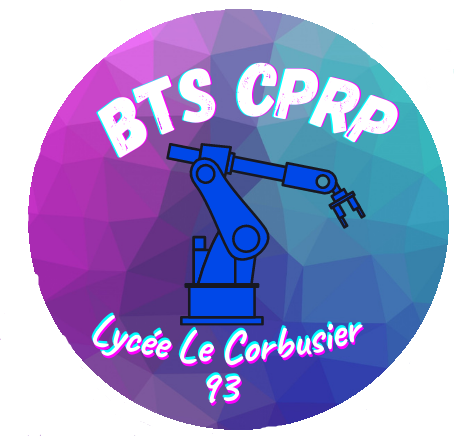
\includegraphics[width=0.2\linewidth]{btscprp.png}}
		\\ [2.0cm]
		\HRule{0.5pt} \\
		\LARGE \textbf{\uppercase{TP1.4 Axes Machines \& architecture des MOCN}}
		\HRule{2pt} \\ [0.5cm]}
\maketitle

\textbf{Deux personnes par groupe}\\
\begin{center}
Toutes les questions seront traitées dans le documents réponse fourni
\end{center}










%-------------------------------------------------------------------------------
% Section title formatting
\sectionfont{\scshape}




\newpage



%%%%%%%%%%%%%%%%%%%%%%%%%%%%%%%%%%%%%%%%%%%%%%%%%%%%%%%%%%%%%%%%
%%%%%%%%%%%%%%%% MACHINE 1 %%%%%%%%%%%%%%%%%%%%%%%%%%%%%%%%%%%%%
%%%%%%%%%%%%%%%%%%%%%%%%%%%%%%%%%%%%%%%%%%%%%%%%%%%%%%%%%%%%%%%%

\tableofcontents
\newpage



\subsection*{Conseils pour le TP:}
\begin{tcolorbox}[colback=blue!5!white,colframe=red!75!black]
  \bcinfo Comme pour tous les TPs, il est conseillé de lire toutes les pages une première fois, comme pour un sujet de BTS. Vous noterez que beaucoup d'informations sont dans les annexes (comme au BTS). Certaines définitions et figures sont "en plus". Avant de poser une question, lisez bien tout le dossier. Ne perdez pas de temps, car les TPs sont conçus pour la durée entière : 3h. En plus de comprendre et apprendre, vous devrez écrire vos réponses au propre. Il vous est fortement conseillé de vous partager le travail entre vous deux.
\end{tcolorbox}


Une machine outil à commande numérique, appelée communément MOCN, est un système
automatisé. Elle est composée d’une partie commande (PC) : le DCN (directeur de commande
numérique) et d’une partie opérative (PO) comprenant la structure de la machine outil, le porte-outil, l’outil et le porte-pièce ; la matière d’oeuvre est la pièce.
\begin{figure}
\centering
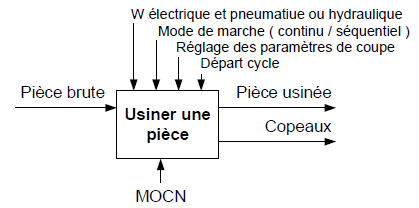
\includegraphics[width=0.7\linewidth]{A0.PNG}
\caption{Analyse fonctionnelle niveau A-0}
\label{A0}
\end{figure}

\newpage

\section{Généralités sur les MOCN}

\begin{minipage}{.55\linewidth}
\textit{Compétences transversales travaillées :}
\begin{itemize}
    \item C1 : Rechercher une information dans une documentation technique, en local ou à distance.
\end{itemize}

\end{minipage}
\begin{minipage}{.44\linewidth}
\textit{Savoirs du programme travaillées :}
\begin{itemize}
    \item S7.4.1 Caractéristiques des machines de production;
    \item S7.4 – Machines.
\end{itemize}
\end{minipage}


\subsection{Machine 1F}

\begin{exo}\label{exo1} A propos de la machine ci-dessous, rayer les mentions inutiles :
\begin{itemize}
    \item C'est une fraiseuse à commande numérique;
    \item C'est un tour à commande numérique;
    \item C'est une perceuse à colonne.
\end{itemize}
\end{exo}


\begin{exo}\label{exo1} Retrouvez les différentes axes, pièces et ensembles constituant la machine-outil à commande numérique (MOCN Figure \ref{MOCN11} \& \ref{MOCN12}) et indiquez les numéros correspondants :\\ \end{exo}
\begin{minipage}{.55\linewidth}
\begin{itemize}
    \item Outil numéro x :
    \item Broche :
    \item Arrosage :
    \item Arrêt d’urgence :
    \item Magasin d’outils :
    \item Directeur de commande numérique :
    \item Porte de sécurité :
\end{itemize}

\end{minipage}
\begin{minipage}{.44\linewidth}
\begin{itemize}
    \item Mandrin :
    \item Bac à copeaux :
    \item Étau :
    \item Axe X :
    \item Outil :
    \item Axe Z :
    \item Bâti :
\end{itemize}
\end{minipage}





%%%%%%%%%%%%%%%%%%%%%% FIN %%%%%%%%%%%%%%%%%%%%%%%%%%%%%%%%%%%%%%%%%%%%%%
%%%%%%%%%%%%%%%%%%%%%%%%%%%%%%%%%%%%%%%%%%%%%%%%%%%%%%%%%%%%%%%%%%%%%%%%%




%%%%%%%%%%%%%%%%%%%%%%%%%%%%%%%%%%%%%%%%%%%%%%%%%%%%%%%%%%%%%%%%
%%%%%%%%%%%%%%%% MACHINE 2 %%%%%%%%%%%%%%%%%%%%%%%%%%%%%%%%%%%%%
%%%%%%%%%%%%%%%%%%%%%%%%%%%%%%%%%%%%%%%%%%%%%%%%%%%%%%%%%%%%%%%%




\subsection{Machine 2T}

\begin{exo}\label{exo1} A propos de la machine ci-dessous, rayer les mentions inutiles :
\begin{itemize}
    \item C'est une fraiseuse à commande numérique;
    \item C'est un tour à commande numérique;
    \item C'est une perceuse à colonne.
\end{itemize}
\end{exo}


\begin{exo}\label{exo1} Retrouvez les différentes axes, pièces et ensembles constituant la machine-outil à commande numérique (MOCN Figure \ref{MOCN21} \& \ref{MOCN22}) et indiquez les numéros correspondants :\\ \end{exo}
\begin{minipage}{.55\linewidth}
\begin{itemize}
    \item Outil numéro x :
    \item Mors :
    \item Mandrin :
    \item Guide chariot vertical $\overrightarrow{x}$ :
    \item Contre-broche :
    \item Centre de commande / pupitre\\ de commande (IHM : Interface homme machine) :
    \item Porte de sécurité :
    \item Axe $\overrightarrow{X}$ :
    \item Bâti :
\end{itemize}


\end{minipage}
\begin{minipage}{.44\linewidth}
\begin{itemize}
    \item Magasin d’outils :
    \item Bac à copeaux :
    \item Marque du constructeur :
    \item Modèle du constructeur :
    \item Bouton d'arrêt d’urgence :
    \item Axe $\overrightarrow{Z}$ :
    \item Axe $\overrightarrow{C}$ :
    \item Axe $\overrightarrow{Y}$ :
\end{itemize}
\end{minipage}

\newpage

\section{Fonctionnement des machines outils}
\textit{Savoirs travaillée : S7.4 – Machines}



\begin{exo}\label{exo1} En vous aidant de la Figure \ref{F1} indiquez d'où viennent les ordres de déplacement des machines outils.\end{exo}
%% D'après la figure, les ordres viennent de la consigne de vitesse dans le directeur de commande (C.N.)

\begin{exo}\label{exo1} Selon le diagramme Figure \ref{F1} de combien d'axe(s) dispose la machine outil  ?\end{exo}
%% De trois axes %%



\begin{exo}\label{exo1} En vous aidant de la Figure \ref{C1} : Que se passe-t-il si, lors d'une erreur de programmation d'usinage, un outil force sur la pièce ?\end{exo}
%% Si un outil force, le couple va augmenter jusqu'à détection du surcouple, la chaîne de sécurité sera alerté et l'automate,  par l'intermédiaire d'une signalisation et du contrôle du variateur, va pouvoir arrêter le processus en cours %%

\section{Structures \& architectures des machines outils}
\textit{Savoirs travaillées :
\begin{itemize}
    \item S7.4.1 – Caractéristiques des machines de production ;
    \item S3.1 – Modélisation des mécanismes ;
    \item S11.1.3 – Structures sérielles et parallèles.
\end{itemize}
 }


La structure articulaire (voir Figure \ref{S1} et Figure \ref{S2}) est le squelette de la machine; il se trouve sous le carter et n'est pas accessible par l'utilisateur. Par analogie au corps humain, nous parlons du squelette de la machine. Ce squelette est composé en général de liaison à \textbf{1 degré de liberté} (articulation) de type \textbf{liaison pivot} (comme notre coude) ou \textbf{liaison glissière} (comme nous, dans un toboggan !).\\



Pour rappel, il existe différentes façon de structurer un système. Des exemples sont visibles sur les \textbf{Figures \ref{Se1}, Figure \ref{Par1}, Figure \ref{Par2} et Figure \ref{Par3}}.

\begin{exo}\label{exo1} En rappelant le nom des machines outils sur lesquelles vous vous êtes rendus, indiquez si, d'après vous, elles font partie d'une structure type \textbf{ouverte} ou \textbf{fermée}. Aidez vous des figures \ref{S1} \& \ref{S2}.\end{exo}

\begin{exo}\label{exo1} Appelez votre enseignant, et inspectez si dans l'atelier de production, vous disposez de machine avec une structure en parallèle.\end{exo}





\section{Système d'axe des machines outil}
\textit{Savoirs travaillées :
\begin{itemize}
    \item S7.4.1 : Système d’axe des machines
    \item S11.1.2 : Machines à 5 axes continus
\end{itemize}
 }

% Aide question : http://philippe.berger2.free.fr/productique/ressources/origines/origines.htm %%%

%% https://fr.calameo.com/read/00087507071e3620cbe22 %%
%% https://fr.calameo.com/books/00087507071e3620cbe22 %%


\subsection{Définition}

\begin{exo}\label{exo1} Rappelez l'intérêt des normes dans l'industrie.\end{exo}


\begin{exo}\label{exo1} Recherchez la définition de la norme \textbf{AFNOR NF Z 68-020}, quel est son but ?\end{exo}


\begin{exo}\label{exo1} En recherchant les informations de la norme \textbf{AFNOR NF Z 68-020}, définissez les notions suivantes :\end{exo}
%% http://philippe.berger2.free.fr/productique/ressources/origines/origines.htm %%
\begin{itemize}
    \item Un axe :
    \item Trièdre de référence : 
    \item Axe $\overrightarrow{Z}$ :\\
\end{itemize}

Pour faire le lien entre les déplacements des axes et le code généré, vous devrez intégrer de nouvelles notions. Nous les travaillerons tout au long des deux années, mais doivent vite être connues pour notamment pouvoir effectuer la FAO (Fabrication Assisté par Ordinateur) sur CATIA.

\begin{exo}\label{exo1} En recherchant les informations de la norme \textbf{AFNOR NF Z 68-021} (attention ce n'est plus la même), définissez les courses et origines suivantes (vous verrez que c'est assez subtile) :\end{exo}
\begin{itemize}
    \item $OM$ :
    \item $Om$ :
    \item $Op$ :
    \item $Opp$ :
    \item PREF :
    \item DEC :
\end{itemize}

\begin{exo}\label{exo66} Parmi les 6 éléments ci-dessus, entourez \textbf{en rouge} ceux qui, selon vous, sont des vecteurs\footnote{Certains de ces éléments sont des points matériels, d'autres sont des distances orientées, des vecteurs. Pour rappel, si vous avez deux origines dans vos machines qui sont : $\vec{O_1} =\begin{pmatrix} 2mm\\0\\5mm \end{pmatrix}$ et $\vec{O_2} =\begin{pmatrix} 1mm\\3mm\\0 \end{pmatrix}$ alors vous pouvez construire un vecteur qui représente la distance entre eux deux : $\overrightarrow{O_1O_2} =\begin{pmatrix} 2 + 1mm\\0 + 3 mm\\5 + 0mm \end{pmatrix}=\begin{pmatrix} 3mm\\3 mm\\5mm \end{pmatrix}$ Et nous pourrions nommer ce vecteur pour qu'il soit plus représentatif de ce que nous voulons :\\ $\overrightarrow{O_1O_2}=\overrightarrow{Dimension De La Piece}=\begin{pmatrix} 3mm\\3 mm\\5mm \end{pmatrix}$ C'est le même principe pour cette question.}(deux éléments attendus).  \end{exo}


\begin{exo}\label{exo1} D'après vous, pour quelle raison principale nous avons eu besoin de définir autant de courses et origines différentes ? \end{exo}
%% Sans ces différentes origines/courses, à chaque changement de pièces, outil, problème quelconque, nous devrions re-régler toute la machine outil. Grâce à elles, on peut facilement changer d'outil et ne changer qu'une seule valeur. Les différents jeu entre les pièces peuvent aussi constamment changer, c'est pourquoi nous avons besoin de beaucoup d'origines différentes. %%




\subsection{Comment dire à la MOCN où commencer votre programme ?}
\subsubsection{Le PREF}
%% http://robert.cireddu.free.fr/Progression/Formation%20en%20PRODUCTIQUE.html %%

\begin{tcolorbox}[colback=blue!5!white,colframe=red!75!black]
  \bcinfo Les machines n'ont pas d'yeux, elles ne peuvent pas "savoir" où sont vos pièces ou vos outils. A la fabrication d'une machine, le constructeur aura déjà entré des paramètres internes nécessaires à son bon fonctionnement -- restera une zone usinable vide et obscure qui n'attend que d'être programmée ! C'est cette zone, totalement noire pour la machine, que vous devez éclairer : lui indiquer où sont ses mains, (les outils) et où se situe la pièce à usiner. Une fois les paramètres connus ( $\overrightarrow{OmOp}$ notamment) la machine pourra faire son job. 
\end{tcolorbox}
% OmOP --> Origine mesure Origine Programme %%
%% Om est le tout premier point, première ref, on ne peut pas le modifier ?

\begin{exo}\label{exo1} Sur les deux figures ci-dessous (vue de coté et vue du dessus), inscrivez \textbf{en rouge} l'origine OP et tracez les distances $\overrightarrow{PREF_X}$, $\overrightarrow{PREF_Y}$ et $\overrightarrow{PREF_Z}$.\end{exo}
\begin{center}
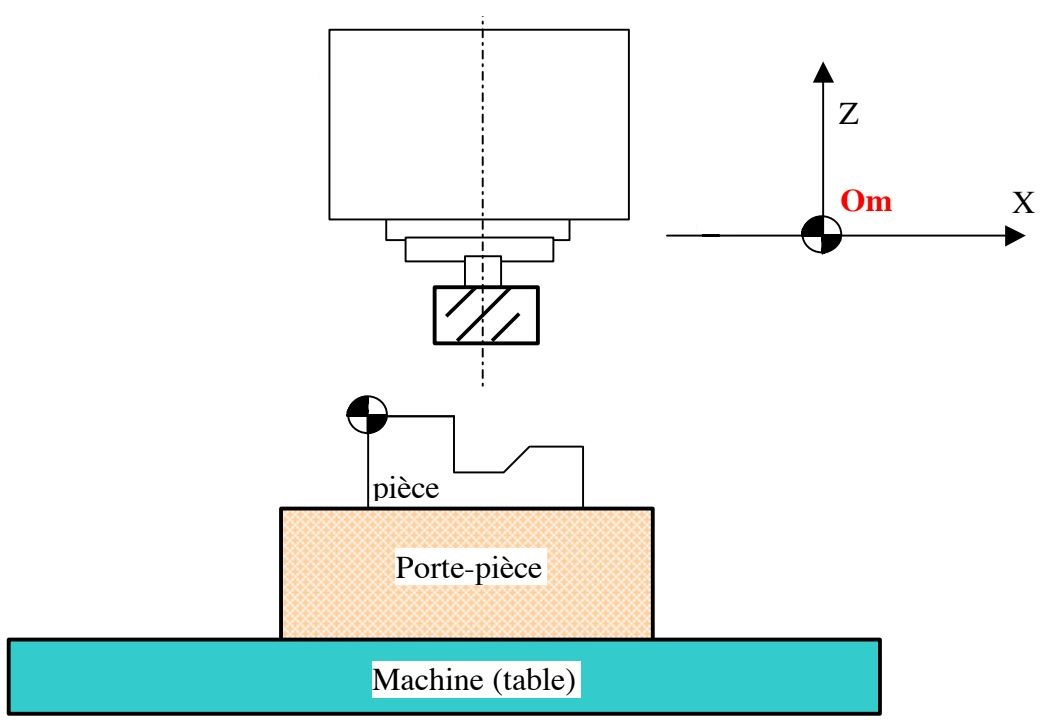
\includegraphics[width=0.8\linewidth]{OmOP1.JPG}
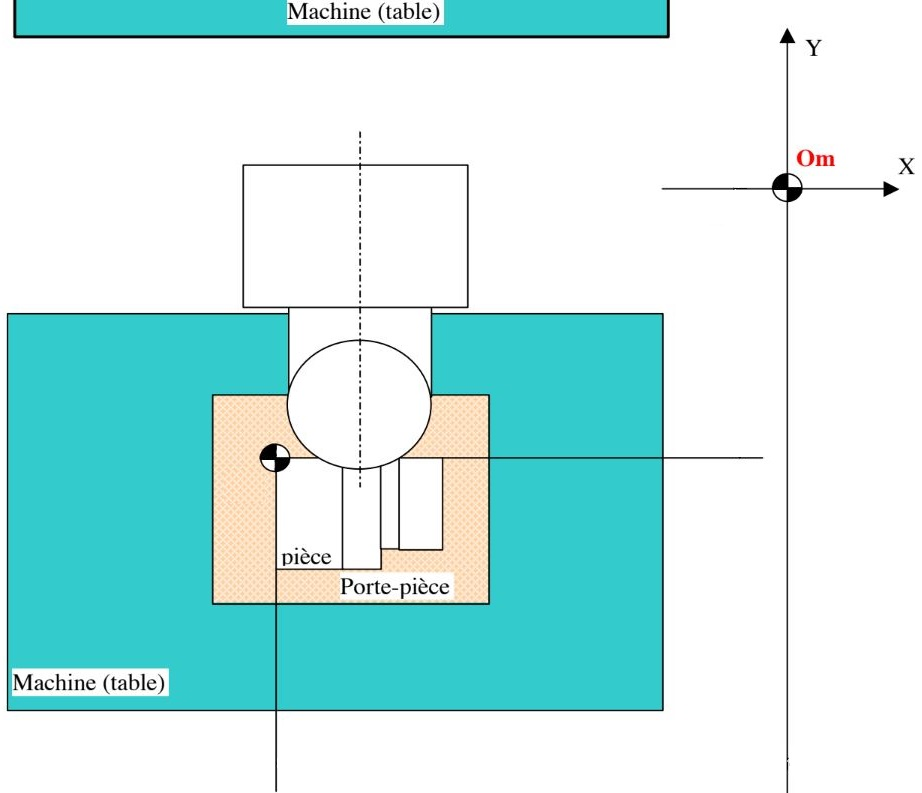
\includegraphics[width=0.8\linewidth]{OmOP2.JPG}
\end{center}

\subsubsection{Le DEC}
\begin{tcolorbox}[colback=blue!5!white,colframe=red!75!black]
  \bcinfo Le $DEC(\vec{x}, \vec{y}, \vec{z})$, c'est un peu comme le vecteur PREF, mais certaines fois il n'est pas utilisé. Par exemple, quand nous ne fabriquons qu'une seule pièce (série unitaire, ou prototype). Cependant, le DEC devient utile quand nous devons usiner plusieurs lots avec des pièces ou porte-pièces différents. Vous êtes en BTS CPRP option sérielle, nous utiliserons donc toujours le DEC.
\end{tcolorbox}


\begin{exo}\label{exo1} Sur les deux figures ci-dessous (vue de coté et vue du dessus), inscrivez \textbf{en rouge} l'origine OP et Opp et tracez les distances $\overrightarrow{PREF_X}$, $\overrightarrow{PREF_Y}$ et $\overrightarrow{PREF_Z}$ ainsi que les $\overrightarrow{DEC_X}$, $\overrightarrow{DEC_Y}$ et $\overrightarrow{DEC_Z}$.\end{exo}
\begin{center}
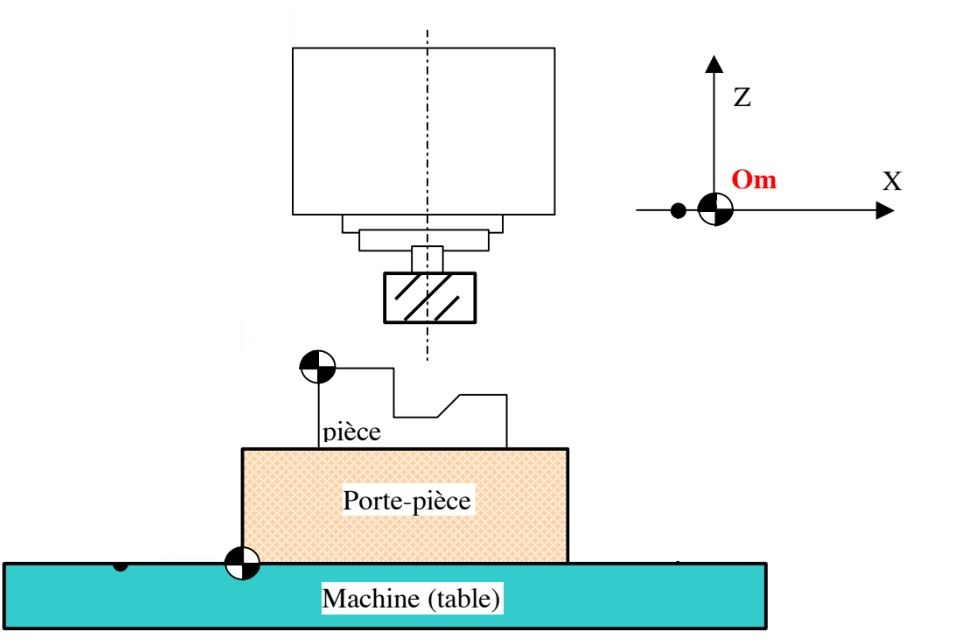
\includegraphics[width=0.8\linewidth]{DEC1.JPG}
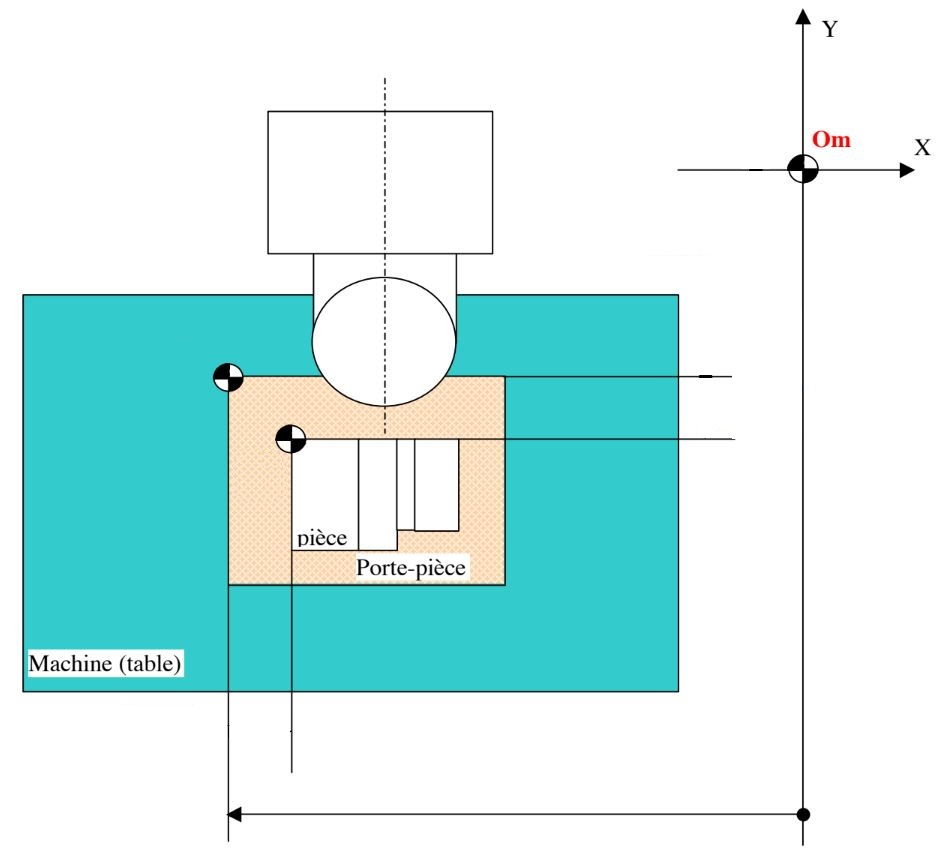
\includegraphics[width=0.85\linewidth]{DEC2.JPG}
\end{center}

\subsection*{En tournage}
Vous devriez avoir compris le principe des PREF et DEC, mais alors, où sont ces origines et vecteurs pour le cas du tournage ?\\
\begin{exo}\label{exo1} Sur la figures ci-dessous, inscrivez \textbf{en rouge} les axes de la machine, l'origine \textbf{OP} et \textbf{Opp} et tracez les distances $\overrightarrow{PREF_X}$, $\overrightarrow{PREF_Y}$ et $\overrightarrow{PREF_Z}$ ainsi que les $\overrightarrow{DEC_X}$, $\overrightarrow{DEC_Y}$ et $\overrightarrow{DEC_Z}$.\end{exo}
\begin{center}
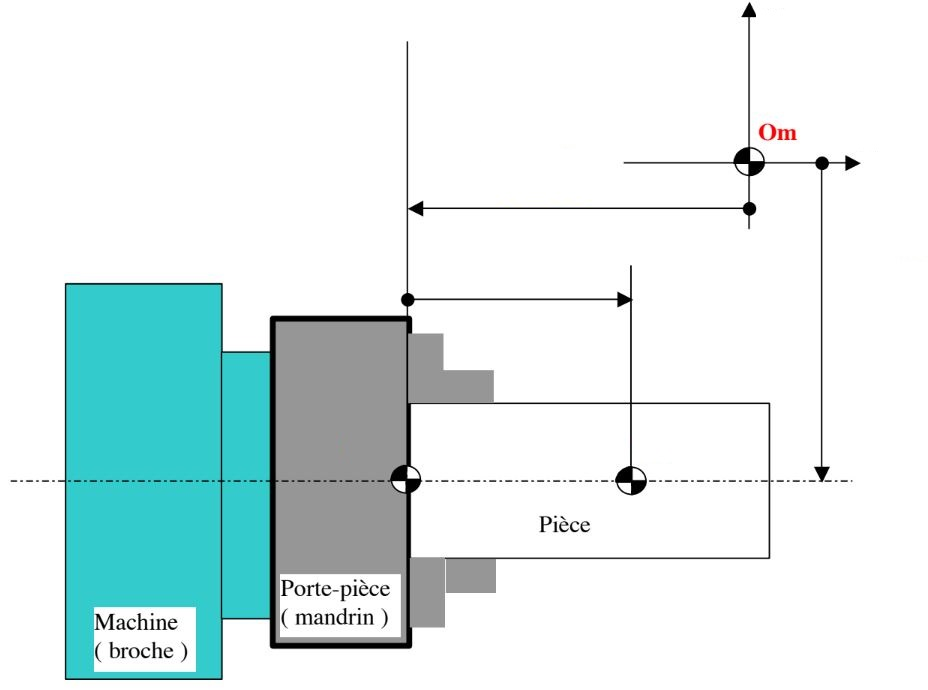
\includegraphics[width=0.9\linewidth]{PREFDEC1.JPG}
\end{center}


\subsection{Comment dire à la MOCN de quelles formes sont vos outils ?}
\begin{tcolorbox}[colback=blue!5!white,colframe=red!75!black]
  \bcinfo Nous avons rendu ses yeux à la machine pour ce qui concerne la pièce, maintenant nous devons lui montrer ses mains (les outils).
\end{tcolorbox}

\subsubsection{Le cas du tournage}
Que sont les \textbf{jauges outil} ? Ce sont les valeurs de longueur de l’outil entre l’origine porte outils et le point générateur (le point qui va usiner). Cette valeur permet de décaler la tourelle afin que ce soit le point générateur qui soit à la position programmée (on a besoin de 2 valeurs, 1 longueur et 1 rayon). Pour définir correctement les jauges outils d’un tour, il faut lui attribuer sa jauge en $\vec{X}$ et en $\vec{Z}$, le
rayon de plaquette R et le cadran de travail pour la correction d’outil.


\begin{exo}\label{exo1} Sur la figures ci-dessous, tracer \textbf{en rouge} les jauges des outils pour le cas d'un tour.\end{exo}
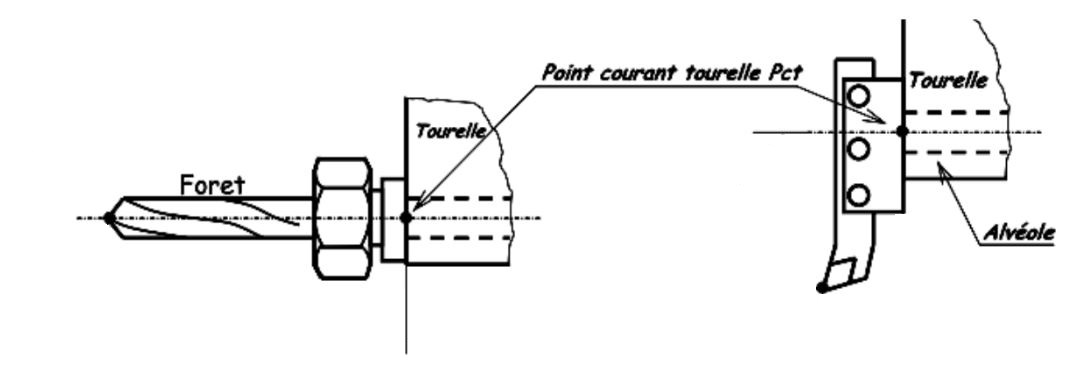
\includegraphics[width=1.05\linewidth]{jauge1.JPG}


\subsubsection{Le cas du fraisage}
Pour définir les jauges d’un outil de fraisage, Il faut lui attribuer une jauge L qui est sa longueur sur $\vec{Z}$, et une jauge R qui est son rayon sur $\vec{X}$ et $\vec{Y}$.


\begin{exo}\label{exo1} Sur la figures ci-dessous, tracer \textbf{en rouge} les jauges des outils pour le cas d'un centre d'usinage.\end{exo}
\begin{center}
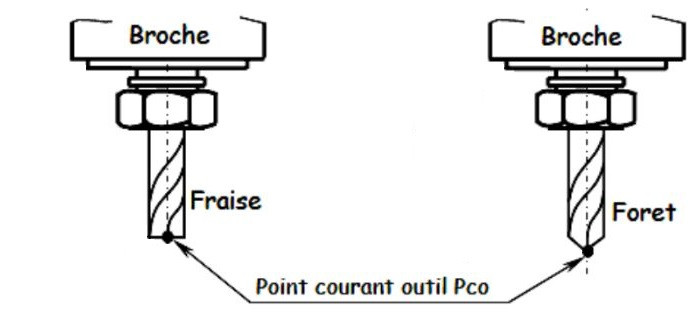
\includegraphics[width=0.8\linewidth]{jauge2.JPG}
\end{center}

Les jauges sont mesurées Statiquement sur un banc de pré-réglage (TP que vous effectuerez en Production) ou effectuées sur la machine. La mesure du rayon de fraise peut s’effectuer à l’extérieur de la machine, ce qui n’inclut pas un
faux rond éventuel du au montage de l’outil dans le porte outil ou à un affûtage défectueux. La mesure de longueur doit toujours tenir compte de l’affûtage de la fraise, il faut prendre la dent la plus longue.\\
Dans le prochain TP nous apprendrons à nommer et identifier les différents outils de production.


%%%%%%%%%%%%%%%%%%%%%%%%%%%%%%%%%%%%%%%%%%%%%%%%%%%%%%%%%%%%%%%%%%%%%%%%%%%%%%%%%%%%%%
%%%%%%%%%%%%%%%%%%%%%%%%%%%%%%%%%%%%%%%%%%%%%%%%%%%%%%%%%%%%%%%%%%%%%%%%%%%%%%%%%%%%%%
%%%%%%%%%%%%%%%%%%%%%%%%%%%%%%%%%%%%%%%%%%%%%%%%%%%%%%%%%%%%%%%%%%%%%%%%%%%%%%%%%%%%%%



%%%%%%%%%%%%%%%%%%%%%%%%%%%%%%%%%%%%%%%%%%%%%%%%%%%%%%%%%%%%%%%%%%%%%%%%%%%%%%%%%%%%%%
%%%%%%%%%%%%%%%%%%%%%%%%%%%%%%%%%%%%%%%%%%%%%%%%%%%%%%%%%%%%%%%%%%%%%%%%%%%%%%%%%%%%%%
%%%%%%%%%%%%%%%%%%%%%%%%%%%%%%%%%%%%%%%%%%%%%%%%%%%%%%%%%%%%%%%%%%%%%%%%%%%%%%%%%%%%%%

\newpage


\section{ANNEXE}
Définitions :
\begin{itemize}
    \item CNC : Computer Numerical Control;
    \item CU : Centre d'usinage;
    \item CAO : Conception Assistée par Ordinateur;
    \item FAO : Fabrication Assistée par Ordinateur.
\end{itemize}



%%%%%%%%%%%%%%%%%%%%%%%%%%%%%%%%%%%%%%%%%%%%%%%%%%%%%%%%%%%%%%%%%%%%%%%%%%%%%%%%%%%%%%
%%%%%%%%%%%%%%%%%%%%%%%%%%%%%%%%%%%%%%%%%%%%%%%%%%%%%%%%%%%%%%%%%%%%%%%%%%%%%%%%%%%%%%
%%%%%%%%%%%%%%%%%%%%%%%%%%%%%%%%%%%%%%%%%%%%%%%%%%%%%%%%%%%%%%%%%%%%%%%%%%%%%%%%%%%%%%
\begin{figure}
\centering
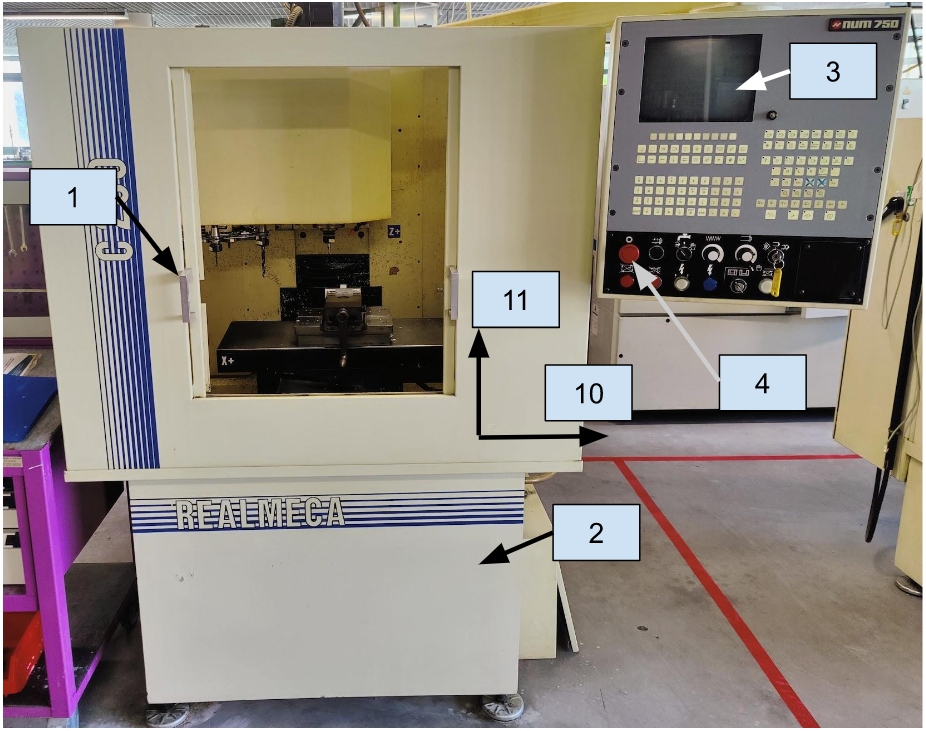
\includegraphics[width=0.7\linewidth]{MOCN11.PNG}
\caption{MOCN 1 - Extérieur}
\label{MOCN11}


\centering
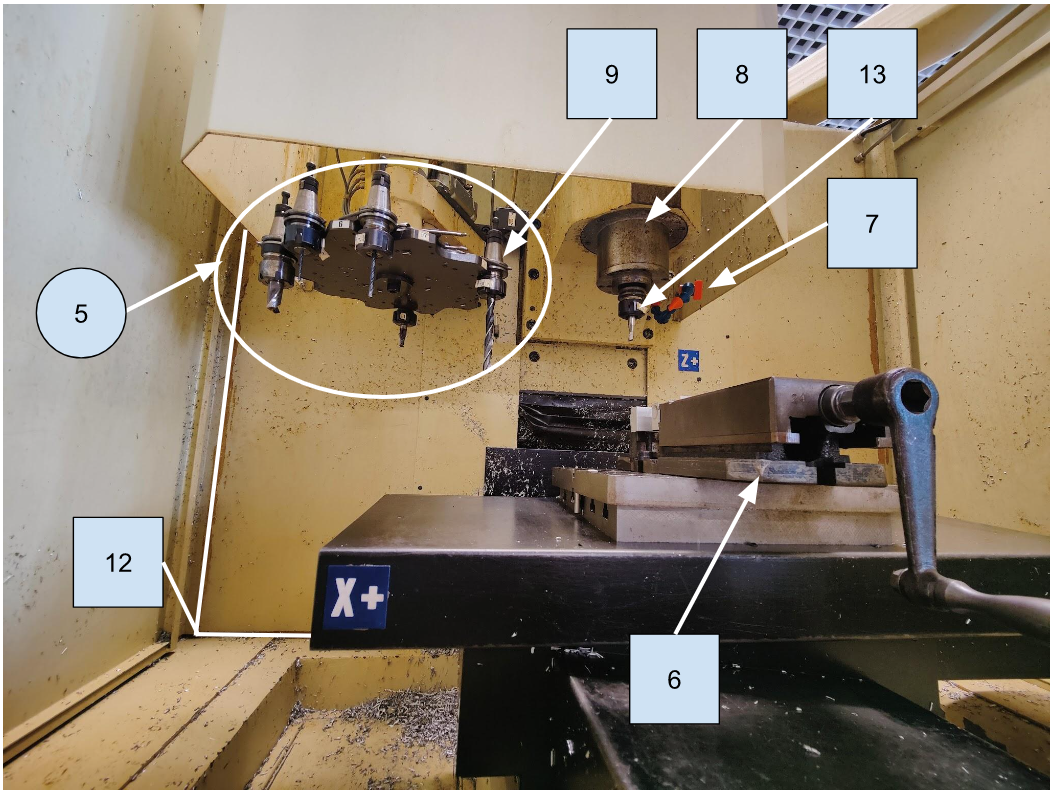
\includegraphics[width=0.7\linewidth]{MOCN12.PNG}
\caption{MOCN 1 - Intérieur}
\label{MOCN12}
\end{figure}
%%%%%%%%%%%%%%%%%%%%%%%%%%%%%%%%%%%%%%%%%%%%%%%%%%%%%%%%%%%%%%%%%%%%%%%%%%%%%%%%%%%%%%
%%%%%%%%%%%%%%%%%%%%%%%%%%%%%%%%%%%%%%%%%%%%%%%%%%%%%%%%%%%%%%%%%%%%%%%%%%%%%%%%%%%%%%
%%%%%%%%%%%%%%%%%%%%%%%%%%%%%%%%%%%%%%%%%%%%%%%%%%%%%%%%%%%%%%%%%%%%%%%%%%%%%%%%%%%%%%

\begin{figure}
\centering
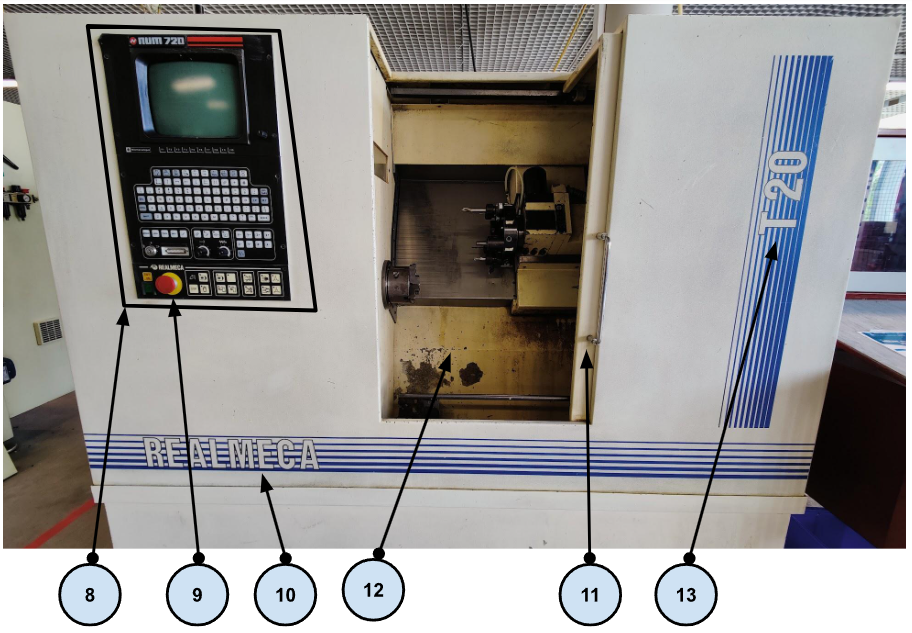
\includegraphics[width=0.75\linewidth]{MOCN21.PNG}
\caption{MOCN 2 - Extérieur}
\label{MOCN21}


\centering
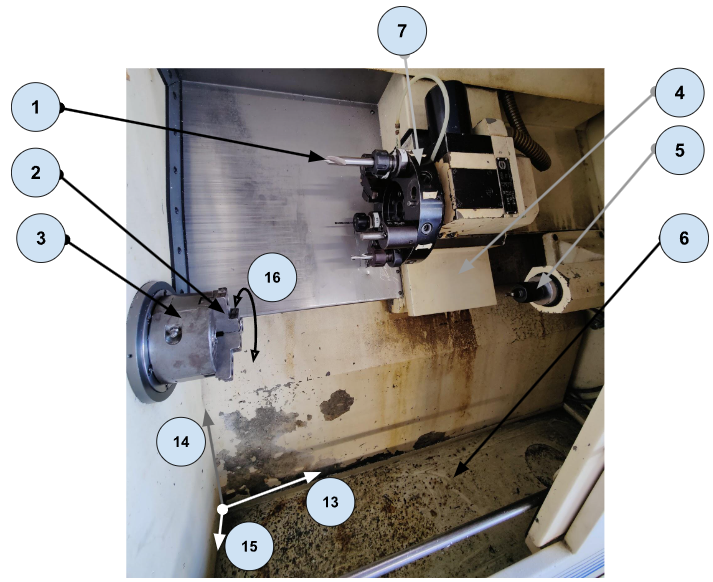
\includegraphics[width=0.75\linewidth]{MOCN22.PNG}
\caption{MOCN 2 - Intérieur}
\label{MOCN22}
\end{figure}
%%%%%%%%%%%%%%%%%%%%%% FIN %%%%%%%%%%%%%%%%%%%%%%%%%%%%%%%%%%%%%%%%%%%%%%
%%%%%%%%%%%%%%%%%%%%%%%%%%%%%%%%%%%%%%%%%%%%%%%%%%%%%%%%%%%%%%%%%%%%%%%%%


\begin{figure}
\centering
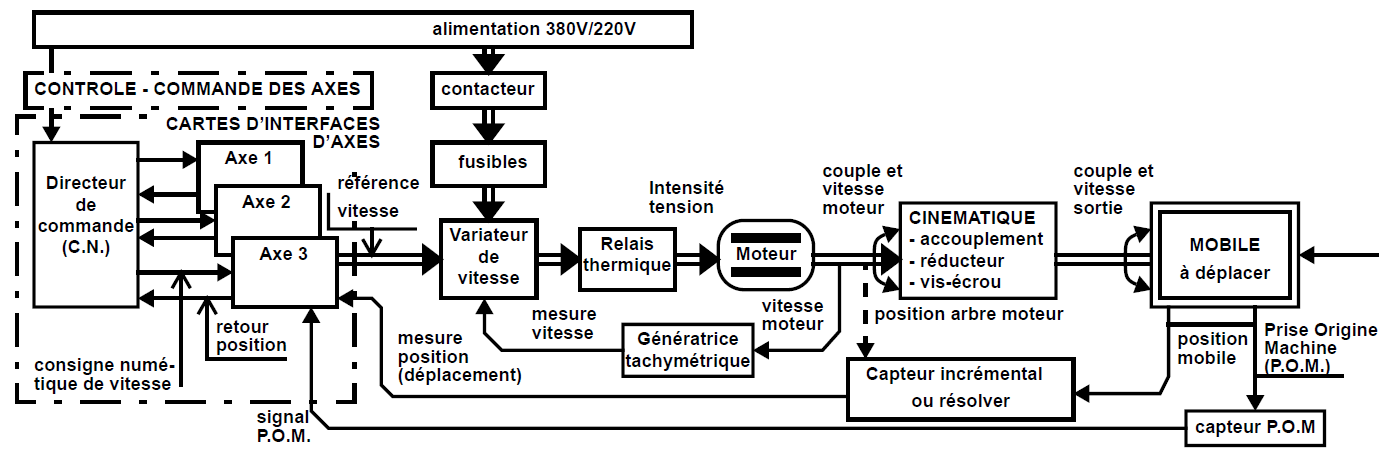
\includegraphics[width=1\linewidth]{fonction1.PNG}
\caption{Fonction contrôle / commande d’une commande d’axe. E.Duc \& E. Lefur.}
\label{F1}
\end{figure}

%%%%%%%%%%%%%%%%%%%%%%%%%%%%%%%%%%%%%%%%%%%%%%%%%%%%%%%%%%%%%%%%%%%%%%%%%%%%%%%%%%%%%%

\begin{figure}
\centering
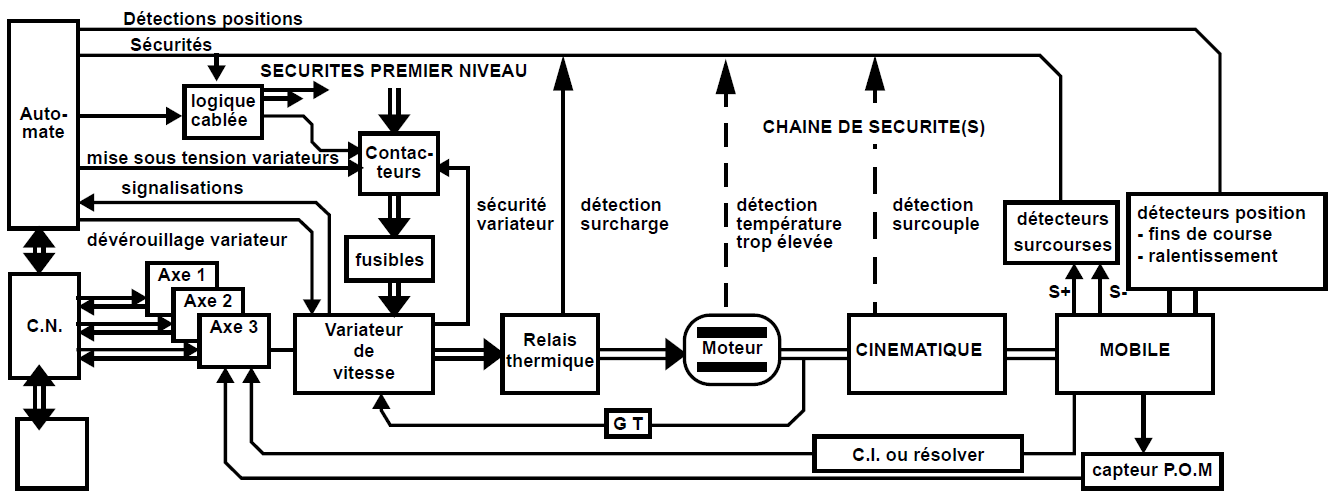
\includegraphics[width=1\linewidth]{conduite1.PNG}
\caption{Fonction conduite / surveillance d’une commande d’axe. E.Duc \& E. Lefur.}
\label{C1}
\end{figure}

%%%%%%%%%%%%%%%%%%%%%%%%%%%%%%%%%%%%%%%%%%%%%%%%%%%%%%%%%%%%%%%%%%%%%%%%%%%%%%%%%%%%%%
%%%%%%%%%%%%%%%%%%%%%%%%%%%%%%%%%%%%%%%%%%%%%%%%%%%%%%%%%%%%%%%%%%%%%%%%%%%%%%%%%%%%%%
%%%%%%%%%%%%%%%%%%%%%%%%%%%%%%%%%%%%%%%%%%%%%%%%%%%%%%%%%%%%%%%%%%%%%%%%%%%%%%%%%%%%%%

\begin{figure}
\begin{minipage}{.55\linewidth}

\centering
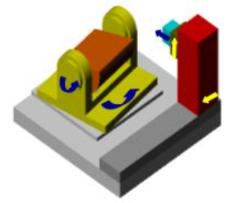
\includegraphics[width=0.6\linewidth]{S1.PNG}
\caption{CU 5 axes, structure à type ouverte.}
\label{S1}

\end{minipage}
\begin{minipage}{.44\linewidth}

\centering
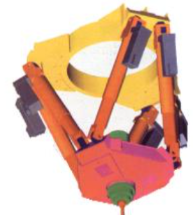
\includegraphics[width=0.6\linewidth]{S2.PNG}
\caption{CU 5 axes, structure à type fermée.}
\label{S2}

\end{minipage}
\end{figure}
%%%%%%%%%%%%%%%%%%%%%%%%%%%%%%%%%%%%%%%%%%%%%%%%%%%%%%%%%%%%%%%%%%%%%%%%%%%%%%%%%%%%%%
%%%%%%%%%%%%%%%%%%%%%%%%%%%%%%%%%%%%%%%%%%%%%%%%%%%%%%%%%%%%%%%%%%%%%%%%%%%%%%%%%%%%%%
%%%%%%%%%%%%%%%%%%%%%%%%%%%%%%%%%%%%%%%%%%%%%%%%%%%%%%%%%%%%%%%%%%%%%%%%%%%%%%%%%%%%%%
\begin{figure}
\centering
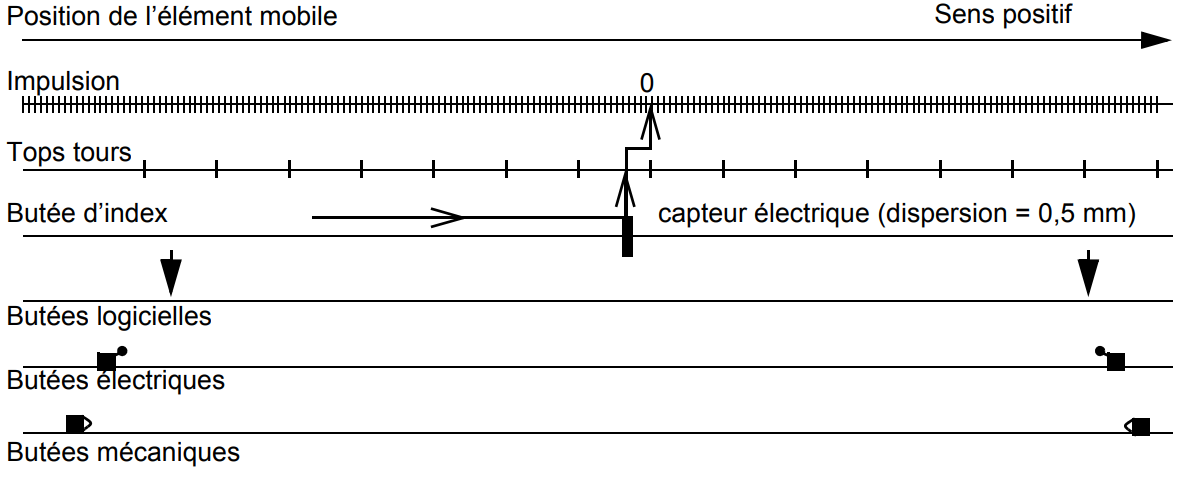
\includegraphics[width=0.85\linewidth]{pos1.PNG}
\caption{Procédure d’initialisation d’un axe numérique pour la prise d'origine machine (POM) (Etienne LEFUR et Christophe SOHIER - Ecole Normale Supérieure de CACHAN.)}
\label{m2}
\end{figure}

%%%%%%%%%%%%%%%%%%%%%%%%%%%%%%%%%%%%%%%%%%%%%%%%%%%%%%%%%%%%%%%%%%%%%%%%%%%%%%%%%%%%%%
%%%%%%%%%%%%%%%%%%%%%%%%%%%%%%%%%%%%%%%%%%%%%%%%%%%%%%%%%%%%%%%%%%%%%%%%%%%%%%%%%%%%%%
%%%%%%%%%%%%%%%%%%%%%%%%%%%%%%%%%%%%%%%%%%%%%%%%%%%%%%%%%%%%%%%%%%%%%%%%%%%%%%%%%%%%%%


\begin{figure}
\begin{minipage}{.55\linewidth}

\centering
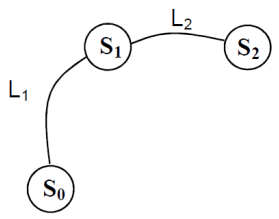
\includegraphics[width=0.7\linewidth]{serie1.PNG}
\caption{Exemple 1.1 : Chaîne de solide en série ouverte.}
\label{Se1}

\end{minipage}
\begin{minipage}{.44\linewidth}

\centering
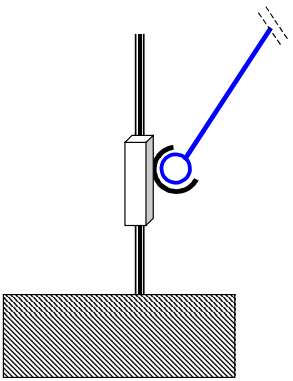
\includegraphics[width=0.7\linewidth]{par1.PNG}
\caption{Exemple 1.2 : Schéma cinématique en série.}
\label{Par1}

\end{minipage}
\end{figure}


%%%%%%%%%%%%%%%%%%%%%%%%%%%%%%%%%%%%%%%%%%%%%%%%%%%%%%%%%%%%%%%%%%%%%%%%%%%%%%%%%%%%%%
%%%%%%%%%%%%%%%%%%%%%%%%%%%%%%%%%%%%%%%%%%%%%%%%%%%%%%%%%%%%%%%%%%%%%%%%%%%%%%%%%%%%%%
%%%%%%%%%%%%%%%%%%%%%%%%%%%%%%%%%%%%%%%%%%%%%%%%%%%%%%%%%%%%%%%%%%%%%%%%%%%%%%%%%%%%%%


\begin{figure}
\begin{minipage}{.55\linewidth}

\centering
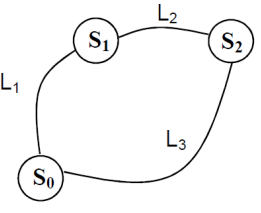
\includegraphics[width=0.7\linewidth]{par2.PNG}
\caption{Exemple 2.1 : Chaîne de solide en parallèle fermée.}
\label{Par2}

\end{minipage}
\begin{minipage}{.44\linewidth}

\centering
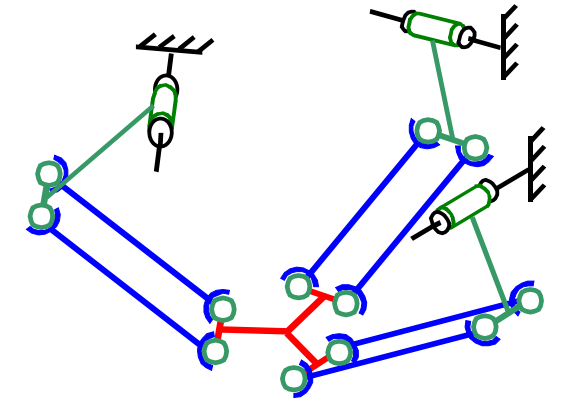
\includegraphics[width=0.8\linewidth]{par3.PNG}
\caption{Exemple 2.2 : Schéma cinématique en parallèle fermée.}
\label{Par3}

\end{minipage}
\end{figure}

%%%%%%%%%%%%%%%%%%%%%%%%%%%%%%%%%%%%%%%%%%%%%%%%%%%%%%%%%%%%%%%%%%%%%%%%%%%%%%%%%%%%%%
%%%%%%%%%%%%%%%%%%%%%%%%%%%%%%%%%%%%%%%%%%%%%%%%%%%%%%%%%%%%%%%%%%%%%%%%%%%%%%%%%%%%%%
%%%%%%%%%%%%%%%%%%%%%%%%%%%%%%%%%%%%%%%%%%%%%%%%%%%%%%%%%%%%%%%%%%%%%%%%%%%%%%%%%%%%%%






%%%%%%%%%%%%%%%%%%%%%%%%%%%%%%%%%%%%%%%%%%%%%%%%%%%%%%%%%%%%%%%%%%%%%%%%%%%%%%%%%%%%%%
%%%%%%%%%%%%%%%%%%%%%%%%%%%%%%%%%%%%%%%%%%%%%%%%%%%%%%%%%%%%%%%%%%%%%%%%%%%%%%%%%%%%%%
%%%%%%%%%%%%%%%%%%%%%%%%%%%%%%%%%%%%%%%%%%%%%%%%%%%%%%%%%%%%%%%%%%%%%%%%%%%%%%%%%%%%%%
\begin{figure}
\centering
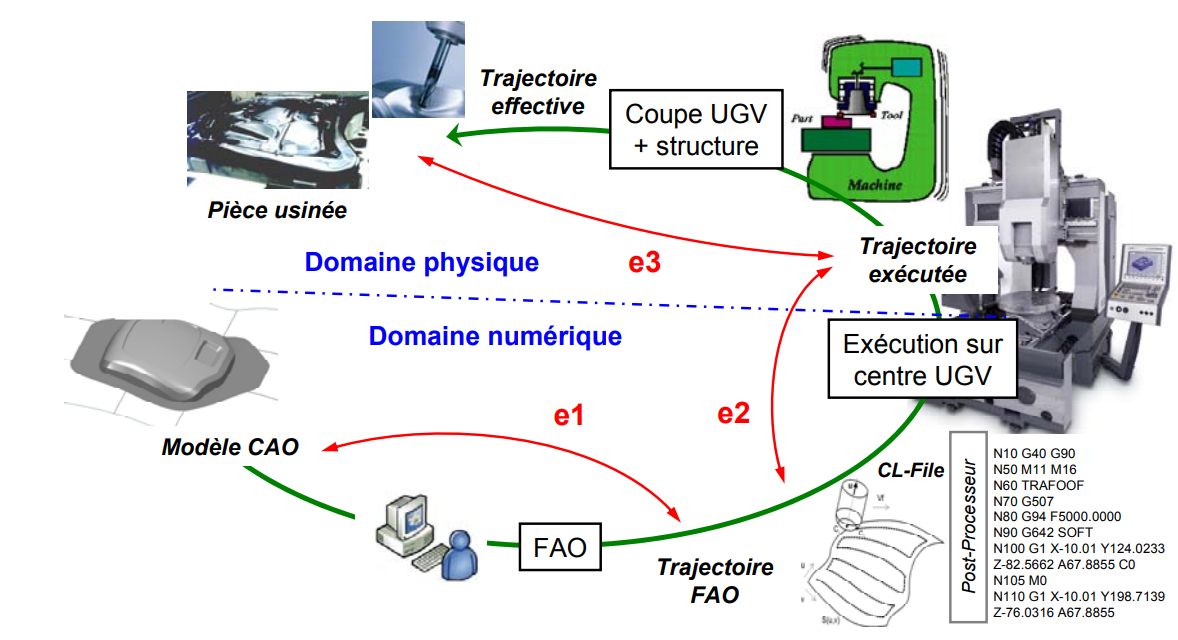
\includegraphics[width=1\linewidth]{mod1.PNG}
\caption{Processus d'élaboration. D.Prévost -- ENS Cachan, 2011}
\label{mod1}
\end{figure}

%%%%%%%%%%%%%%%%%%%%%%%%%%%%%%%%%%%%%%%%%%%%%%%%%%%%%%%%%%%%%%%%%%%%%%%%%%%%%%%%%%%%%%
%%%%%%%%%%%%%%%%%%%%%%%%%%%%%%%%%%%%%%%%%%%%%%%%%%%%%%%%%%%%%%%%%%%%%%%%%%%%%%%%%%%%%%
%%%%%%%%%%%%%%%%%%%%%%%%%%%%%%%%%%%%%%%%%%%%%%%%%%%%%%%%%%%%%%%%%%%%%%%%%%%%%%%%%%%%%%





%%%%%%%%%%%%%%%%%%%%%%%%%%%%%%%%%%%%%%%%%%%%%%%%%%%%%%%%%%%%%%%%%%%%%%%%%%%%%%%%%%%%%%
%%%%%%%%%%%%%%%%%%%%%%%%%%%%%%%%%%%%%%%%%%%%%%%%%%%%%%%%%%%%%%%%%%%%%%%%%%%%%%%%%%%%%%
%%%%%%%%%%%%%%%%%%%%%%%%%%%%%%%%%%%%%%%%%%%%%%%%%%%%%%%%%%%%%%%%%%%%%%%%%%%%%%%%%%%%%%


%%%%%%%%%%%%%%%%%%%%%%%%%%%%%%%%%%%%%%%%%%%%%%%%%%%%%%%%%%%%%%%%%%%%%%%%%%%%%%%%%%%%%%
%%%%%%%%%%%%%%%%%%%%%%%%%%%%%%%%%%%%%%%%%%%%%%%%%%%%%%%%%%%%%%%%%%%%%%%%%%%%%%%%%%%%%%
%%%%%%%%%%%%%%%%%%%%%%%%%%%%%%%%%%%%%%%%%%%%%%%%%%%%%%%%%%%%%%%%%%%%%%%%%%%%%%%%%%%%%%


%%%%%%%%%%%%%%%%%%%%%%%%%%%%%%%%%%%%%%%%%%%%%%%%%%%%%%%%%%%%%%%%%%%%%%%%%%%%%%%%%%%%%%
%%%%%%%%%%%%%%%%%%%%%%%%%%%%%%%%%%%%%%%%%%%%%%%%%%%%%%%%%%%%%%%%%%%%%%%%%%%%%%%%%%%%%%
%%%%%%%%%%%%%%%%%%%%%%%%%%%%%%%%%%%%%%%%%%%%%%%%%%%%%%%%%%%%%%%%%%%%%%%%%%%%%%%%%%%%%%








\end{document}

